\documentclass[../main.tex]{subfiles}

\begin{document}

\chapter{Теоретичні відомості та аналітика}

\section{Призначення та область застосування об'єкта проектування}

Люди, які часто подорожують відвідують багато різних місць, зустрічаються з новими людьми, переживають нові ситуації. Деякі події залишаються в пам'яті, деякі відходять на другий план попри небажання їх забути. Інформація накопичується, а людина не в змозі запам'ятати все. Тому, необхідність збереження пам'яті про деякі події, місця чи враження зумовлює створення систем для задоволення таких потреб.

Призначення щоденників полягає в тому, щоб зберігати записи за певний період часу. 

\section{Способи та засоби реалізації}

Так як щоденник є мобільним Android додатком, то для його розробки актуальними є такі мови програмування як Java чи Kotlin. 

\begin{itemize}
    \item Java – строго типізована об'єктно-орієнтована мова програмування. Програми Java зазвичай транслюються в спеціальний байт-код, тому вони можуть працювати на будь-якої комп'ютерної архітектурі, за допомогою віртуальної Java-машини.
    \item Kotlin – статично типізована мова програмування, що працює поверх JVM і розробляється компанією JetBrains. Компілюється також в JavaScript. Автори ставили за мету створити мову більш лаконічну та типо-безпечнішу, ніж Java, та простішу, ніж Scala.
\end{itemize}

Ці мови програмування є об'єктно-орієнтованими, та сама Android SDK (універсальний засіб розробки мобільних додатків для операційної системи Android) базується на цих принципах, тому написання Android-додатку неможливе без використання ООП. Об'єктно-орієнтоване програмування – це методологія програмування, заснована на представленні програми у вигляді сукупності об'єктів, кожен з яких є екземпляром певного класу, а класи утворюють ієрархію спадкування.

Останнім часом для збереження даних в Android-додатках активно використовують бази даних noSQL, такі як Realm чи Firebase. В нашому випадку потрібна також синхронізація між пристроями, тому актуальним вибором є Firebase, так як вона також являє собою базу даних, яка в реальному часі поновлює інформацію на всіх з'єднаних з нею пристроях. Також плюсом цієї БД є те, що вона зберігає дані оффлайн на пристрої, тому при втраті інтернет з'єднання всі дані будуть збережені і вивантажені при його відновленні.

Для авторизації користувачів в додатку зручним та актуальним способом є авторизація за допомогою Google-аккаунта. Більшість Android користувачів мають його, тому їм не доведеться створювати нові аккаунти та запам'ятовувати новий пароль.

Найпопулярнішим та офіційним середовищем розробки для Android є Android Studio. 
Воно дозволяє швидко та зручно писати код, збирати проекти за допомогою Gradle (система автоматичного збирання, побудована на принципах Apache Ant і Apache Mave).

В додатку наявний запис треку переміщень. Всі сучасні смартфони обладнані GPS-приймачем, тому вони можуть виступати в ролі трекера.  Як окремий пристрій GPS-трекер являє собою прилад прийому-передачі даних для супутникового контролю автомобілей, людей чи інших об'єктів, до яких він прикріплюється, що використовує GPS для точного визначення місцезнаходження об'єкта. Глобальна система позиціонування (GPS) – супутникова система навігації, що забезпечує вимір відстані, часу та визначає місцезнаходження у всесвітній системі координат WGS 84. Дозволяє в будь-якому місці Землі визначати місцезнаходження та швидкість об'єктів. Вона також потрібна для реалізації нагадувань по приближенню до заданого місця.

\section{Аналіз переваг та недоліків програм аналогів}

Існує багато різноманітних додатків, які являють собою Android-щоденники для мандрівників, розглянемо більш детально основні з них.

Першим розглянутим продуктом є Journey - Diary, Journal від розробника Two App Studio Pte. Ltd. Додаток містить обов'язкову авторизацію за допомогою аккаунту Google. Можна створювати записи, вказувати для них теги та додавати до 4-х фото. При вказанні локації автоматично завантажуються дані про погоду. Також можна вказувати активність (непорушний, біг, політ і тд.). Для користування можливостями розмітки «Markdown» потрібно купувати преміум-аккаунт. Головний екран додатку містить список записів (див. рис. \ref{figure:1}). Присутній пошук, але він фільтрує тільки по тексту запису. Синхронізація даних відбувається через Google Drive (сховище даних, що дозволяє користувачам зберігати свої дані на серверах у хмарі і ділитися ними з іншими користувачами в Інтернеті). Також є можливість поділитися та опублікувати запис. 

\hfill

\begin{figure}[H]
\centering
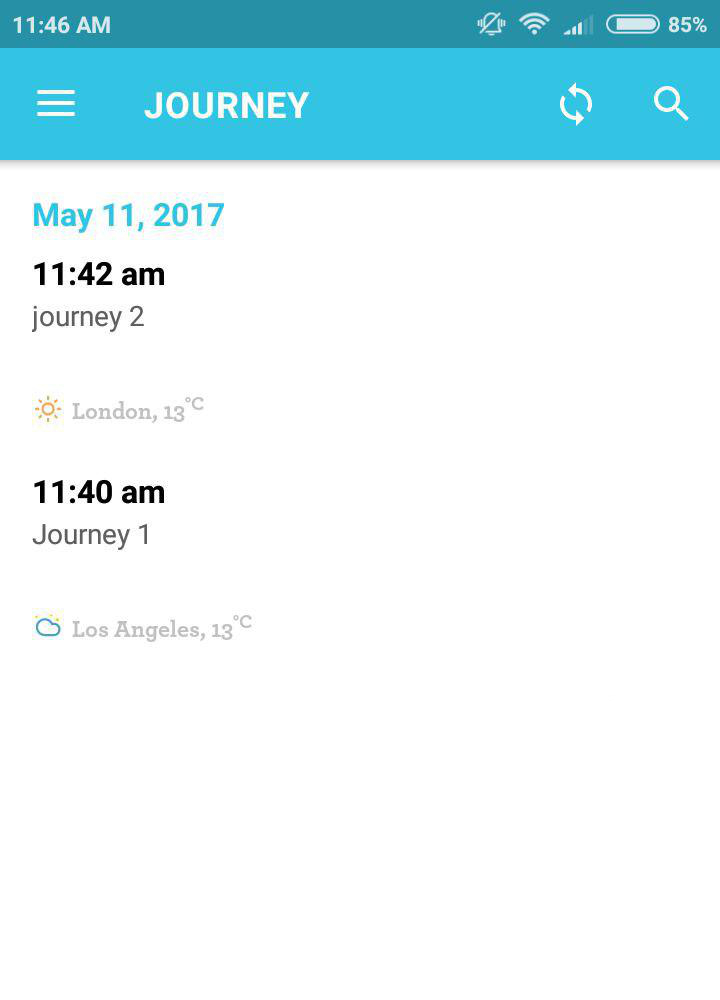
\includegraphics[width=0.35\textwidth]{journey_main_screen}
\caption{Головний екран додатку Journey - Diary, Journal}
\label{figure:1}
\end{figure}

\break
Наступним продуктом є Travel Diary від розробника Tristan Rücker. Додаток являє собою записник, в якому можна створювати категорії (подорожі). Головний екран містить список цих подорожей (див. рис. \ref{figure:2}). Логотип подорожі користувач вказує сам, обираючи один із трьох доступних. В категоріях можна робити записи, прикріпляти до них фото та вказувати локації. Ці записи можна експортувати в pdf-файли, надсилати через електронну пошту. Також можна переглядати вказані локації на карті, але лише для одного запису. Присутнє сортування записів за датою та назвою.

\hfill

\begin{figure}[H]
\centering
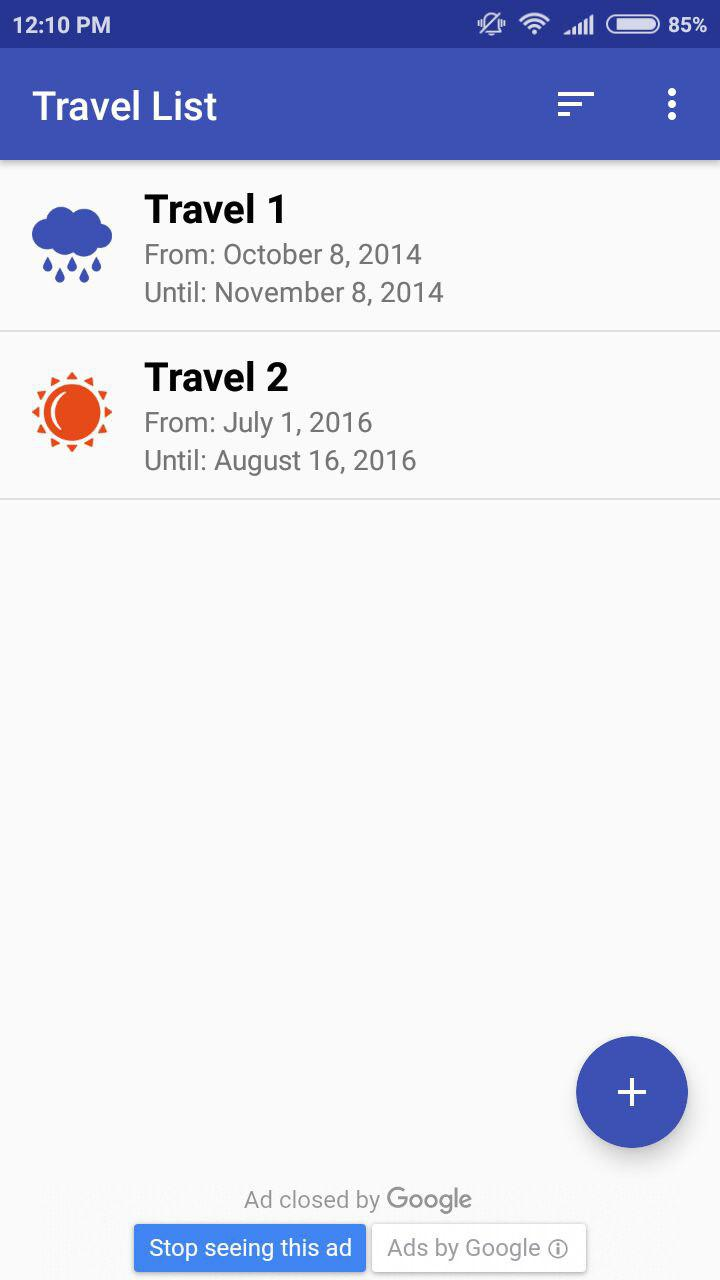
\includegraphics[width=0.35\textwidth]{travel_diary_main_screen}
\caption{Головний екран додатку Travel Diary}
\label{figure:2}
\end{figure}

\hfill

Ще одним розглянутим продуктом є Universal diary від розробника SPB Apps. Головний екран містить календар, потрібно обрати дату для того щоб продовжити (див. рис. \ref{figure:3}). Після обрання дати можна створювати записи, так звані мітки дня. Міткою дня може бути текст, фото, задача чи фінанси. Можливе створення резервної копії на Google Drive чи на карті пам'яті. При спробі виходу з додатку декілька раз показується реклама.

\begin{figure}[H]
\centering
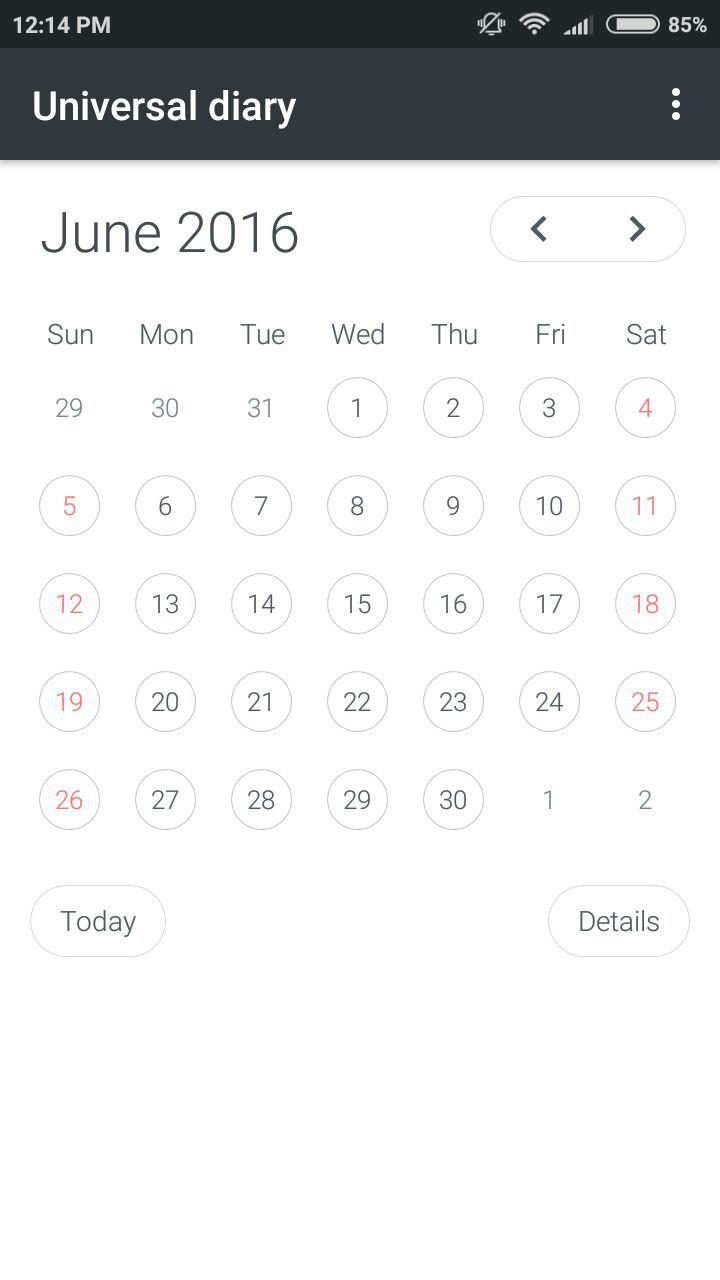
\includegraphics[width=0.35\textwidth]{universal_diary_main_screen}
\caption{Головний екран додатку Universal diary}
\label{figure:3}
\end{figure}

Отже, порівняння основних функцій додатків аналогів та додатку за темою дипломної роботи буде виглядати так, як вказано в таблиці \ref{table:1}.

\begin{center}
\begin{tabular}{ |p{2.5cm}|p{2cm}|p{2.5cm}|p{2.5cm}|p{2.5cm}|p{2.5cm}| } 
    \hline
    \thead{Назва} &
    \thead{Щоденник} &
    \thead{Нагадування\\за часом} &
    \thead{Нагадування\\за місцем} &
    \thead{Запис треку\\переміщень} &
    \thead{Синхронізація} \\
    \hline
    Journey &
    \thead{+} &
    & & &
    \thead{+} \\
    \hline
    Travel Diary &
    \thead{+} &
    & & & \\    
    \hline
    Universal diary &
    \thead{+} &
    \thead{+} & 
    & & \\
    \hline
    Розроблюваний додаток &
    \thead{+} &
    \thead{+} & 
    \thead{+} & 
    \thead{+} & 
    \thead{+} \\
    \hline
\end{tabular}
\captionof{table}{Порівняльна таблиця основних функцій існуючих додатків аналогів}
\label{table:1}
\end{center}

\break
Порівняємо також додаткові функції цих додатків. Результати представлено в таблиці \ref{table:2}.

\begin{center}
\begin{tabular}{ |p{2.5cm}|p{2cm}|p{2.5cm}|p{2.5cm}|p{2.5cm}|p{2.5cm}| } 
    \hline
    \thead{Назва} &
    \thead{Додавання\\фото} &
    \thead{Місце\\свотрення\\запису} &
    \thead{Збереження\\погодних умов} &
    \thead{Експорт\\записів} &
    \thead{Створення\\резервної копії} \\
    \hline
    Journey &
    \thead{+} &
    \thead{+} & 
    \thead{+} & 
    \thead{+} & \\
    \hline
    Travel Diary &
    \thead{+} &
    \thead{+} &
    & & 
    \thead{+} \\    
    \hline
    Universal diary &
    \thead{+} &
    & & & 
    \thead{+}\\
    \hline
    Розроблюваний додаток &
    \thead{+} &
    \thead{+} & 
    \thead{+} & 
    & \\
    \hline
\end{tabular}
\captionof{table}{Порівняльна таблиця додаткових функцій існуючих додатків аналогів}
\label{table:2}
\end{center}

Порівнявши функції додатків, бачимо, що розроблюваний додаток об'єднує в собі як функції які є окремо в додатках аналогах, так і додаткові функції, такі як запис треку, чи нагадування за місцем.

\section{Задача розробки}

Програмних продуктів, які дозволяють вести щоденник, досить багато. Існують також додатки окремо для запису треку переміщень чи встановлення нагадувань, але продуктів, що поєднують в собі ці функції не так багато.
Щоб відповідати сучасним вимогам розробки програмного забезпечення, майбутній продукт повинен задовольняти такі вимоги: 

\begin{itemize}
	\item Можливість створення/редагування/видалення подорожі
	\item Можливість створення/редагування/видалення запису щоденника та планувальника
	\item Можливість додавання/видалення фото в записі щоденника
	\item Зберігання погодних умов та місця сворення запису
	\item Можливість ділитися записом щоденника та окремими фото
	\item Можливість запису треку переміщень та перегляду його на карті
	\item Можливість створення/редагування/видалення списку завдань та нагадувань (планувальника)
\end{itemize}

Практичною цінністю майбутнього додатку є надання комплесу інструментів для допомоги в організації та збереженні вражень від подорожей чи плануванні майбутніх поїздок.

\end{document}